\documentclass[journal,12pt,twocolumn]{IEEEtran}
%
\usepackage{setspace}
\usepackage{gensymb}
%\doublespacing
\singlespacing

\usepackage{graphicx}
\usepackage[cmex10]{amsmath}
\usepackage{amsmath,amsthm}
\usepackage{mathrsfs}
\usepackage{txfonts}
\usepackage{stfloats}
\usepackage{bm}
\usepackage{cite}
\usepackage{cases}
\usepackage{subfig}

\usepackage{longtable}
\usepackage{multirow}
\usepackage{commath}
\usepackage{enumitem}
\usepackage{mathtools}
\usepackage{steinmetz}
\usepackage{tikz}
\usepackage{circuitikz}
\usepackage{verbatim}
\usepackage{tfrupee}
\usepackage[breaklinks=true]{hyperref}

\usepackage{tkz-euclide}

\usetikzlibrary{calc,math}
\usepackage{listings}
\usepackage{color}                                            
\usepackage{array}                                            
\usepackage{longtable}                                        
\usepackage{calc}                                             
\usepackage{multirow}                                         
\usepackage{hhline}                                           
\usepackage{ifthen}                                           
\usepackage{lscape}     
\usepackage{multicol}
\usepackage{chngcntr}

\DeclareMathOperator*{\Res}{Res}

\renewcommand\thesection{\arabic{section}}
\renewcommand\thesubsection{\thesection.\arabic{subsection}}
\renewcommand\thesubsubsection{\thesubsection.\arabic{subsubsection}}

\renewcommand\thesectiondis{\arabic{section}}
\renewcommand\thesubsectiondis{\thesectiondis.\arabic{subsection}}
\renewcommand\thesubsubsectiondis{\thesubsectiondis.\arabic{subsubsection}}

\hyphenation{op-tical net-works semi-conduc-tor}
\def\inputGnumericTable{}                                 

\lstset{
	%language=C,
	frame=single, 
	breaklines=true,
	columns=fullflexible
}
\lstset{
	%language=TeX,
	frame=single, 
	breaklines=true
}

\begin{document}
	
	
	\newtheorem{theorem}{Theorem}[section]
	\newtheorem{problem}{Problem}
	\newtheorem{proposition}{Proposition}[section]
	\newtheorem{lemma}{Lemma}[section]
	\newtheorem{corollary}[theorem]{Corollary}
	\newtheorem{example}{Example}[section]
	\newtheorem{definition}[problem]{Definition}
	
	\newcommand{\BEQA}{\begin{eqnarray}}
		\newcommand{\EEQA}{\end{eqnarray}}
	\newcommand{\define}{\stackrel{\triangle}{=}}
	\bibliographystyle{IEEEtran}
	\providecommand{\mbf}{\mathbf}
	\providecommand{\pr}[1]{\ensuremath{\Pr\left(#1\right)}}
	\providecommand{\qfunc}[1]{\ensuremath{Q\left(#1\right)}}
	\providecommand{\sbrak}[1]{\ensuremath{{}\left[#1\right]}}
	\providecommand{\lsbrak}[1]{\ensuremath{{}\left[#1\right.}}
	\providecommand{\rsbrak}[1]{\ensuremath{{}\left.#1\right]}}
	\providecommand{\brak}[1]{\ensuremath{\left(#1\right)}}
	\providecommand{\lbrak}[1]{\ensuremath{\left(#1\right.}}
	\providecommand{\rbrak}[1]{\ensuremath{\left.#1\right)}}
	\providecommand{\cbrak}[1]{\ensuremath{\left\{#1\right\}}}
	\providecommand{\lcbrak}[1]{\ensuremath{\left\{#1\right.}}
	\providecommand{\rcbrak}[1]{\ensuremath{\left.#1\right\}}}
	\theoremstyle{remark}
	\newtheorem{rem}{Remark}
	\newcommand{\sgn}{\mathop{\mathrm{sgn}}}
	\providecommand{\abs}[1]{\(\left\vert#1\right\vert\)}
	\providecommand{\res}[1]{\Res\displaylimits_{#1}} 
	\providecommand{\norm}[1]{\(\left\lVert#1\right\rVert\)}
	%\providecommand{\norm}[1]{\lVert#1\rVert}
	\providecommand{\mtx}[1]{\mathbf{#1}}
	\providecommand{\mean}[1]{E\(\left[ #1 \right]\)}
	\providecommand{\fourier}{\overset{\mathcal{F}}{ \rightleftharpoons}}
	%\providecommand{\hilbert}{\overset{\mathcal{H}}{ \rightleftharpoons}}
	\providecommand{\system}{\overset{\mathcal{H}}{ \longleftrightarrow}}
	%\newcommand{\solution}[2]{\textbf{Solution:}{#1}}
	\newcommand{\solution}{\noindent \textbf{Solution: }}
	\newcommand{\cosec}{\,\text{cosec}\,}
	\providecommand{\dec}[2]{\ensuremath{\overset{#1}{\underset{#2}{\gtrless}}}}
	\newcommand{\myvec}[1]{\ensuremath{\begin{psmallmatrix}#1\end{psmallmatrix}}}
	\newcommand{\mydet}[1]{\ensuremath{\begin{vmatrix}#1\end{vmatrix}}}
	%\numberwithin{equation}{section}
	\numberwithin{equation}{subsection}
	%\numberwithin{problem}{section}
	%\numberwithin{definition}{section}
	\makeatletter
	\@addtoreset{figure}{problem}
	\makeatother
	\let\StandardTheFigure\thefigure
	\let\vec\mathbf
	%\renewcommand{\thefigure}{\theproblem.\arabic{figure}}
	\renewcommand{\thefigure}{\theproblem}
	%\setlist[enumerate,1]{before=\renewcommand\theequation{\theenumi.\arabic{equation}}
	%\counterwithin{equation}{enumi}
	%\renewcommand{\theequation}{\arabic{subsection}.\arabic{equation}}
	\def\putbox#1#2#3{\makebox[0in][l]{\makebox[#1][l]{}\raisebox{\baselineskip}[0in][0in]{\raisebox{#2}[0in][0in]{#3}}}}
	\def\rightbox#1{\makebox[0in][r]{#1}}
	\def\centbox#1{\makebox[0in]{#1}}
	\def\topbox#1{\raisebox{-\baselineskip}[0in][0in]{#1}}
	\def\midbox#1{\raisebox{-0.5\baselineskip}[0in][0in]{#1}}
	\vspace{3cm}
	\title{Assignment 4}
	\author{Addagalla Satyanarayana}
	\maketitle
	\newpage
	%\tableofcontents
	\bigskip
	\renewcommand{\thefigure}{\theenumi}
	\renewcommand{\thetable}{\theenumi}
\begin{abstract}
This document uses the properties of a tangent to a circle
\end{abstract}
Download latex-tikz codes from 
%
\begin{lstlisting}
https://github.com/AddagallaSatyanarayana/AI5006/tree/master/Assignment4/Assignment4.tex
\end{lstlisting}
%
\section{Problem}
Find the length of the tangent from the point $\myvec{7\\4}$ to the circle
\begin{align}
		 \vec{x}^T\vec{x}- \myvec{4 & 6}\vec{x}+12=0\label{eq:1}
\end{align}
\section{Explanation}
The general equation of a second degree can be expressed as :
\begin{align}
	\vec{x}^T\vec{V}\vec{x}+2\vec{u}^T\vec{x}+f=0\label{gen__quad_eqn}
\end{align}
Let the point of intersection of the tangent and the circle be denoted by $\vec{p}$ as shown in figure below.

\begin{figure}[!ht]
	\centering
	\resizebox{\columnwidth}{!}{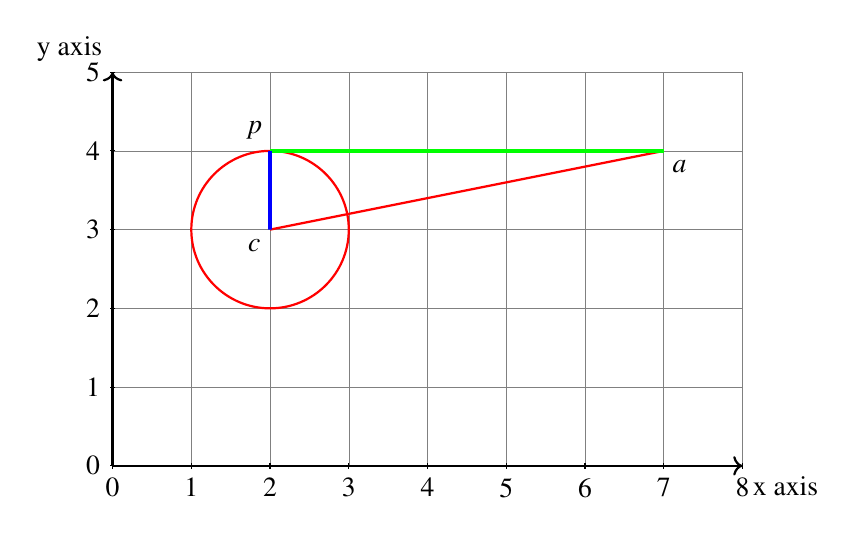
\begin{tikzpicture}
[
	scale=1,
	point/.style = {draw, circle, fill=green, inner sep=0.5pt},
]
\draw[step=1cm,gray,very thin] (0,0) grid (8,5);		

\draw[red,thick] (2,3) circle (1 cm);
\draw (1.8,3) node[anchor=north]{$c$};		
\draw (1.8,4.5) node[anchor=north]{$p$};


\draw (7.2,4) node[anchor=north]{$a$};
\draw[red][thick] (2,3) -- (7,4) 	-- cycle;
\draw[green][very thick] (2,4) -- (7,4) 	-- cycle;
\draw[blue][very thick] (2,3) -- (2,4) 	-- cycle;	
	
\draw[thick,->] (0,0) -- (8,0) node[anchor=north west] {x axis};
\draw[thick,->] (0,0) -- (0,5) node[anchor=south east] {y axis};
\foreach \x in {0,1,2,3,4,5,6,7,8}
\draw (\x cm,1pt) -- (\x cm,-1pt) node[anchor=north] {$\x$};
\foreach \y in {0,1,2,3,4,5}
\draw (1pt,\y cm) -- (-1pt,\y cm) node[anchor=east] {$\y$};
\end{tikzpicture}
}
	\caption{Tangent to Circle }
	\label{fig1:Circle-tangent}
\end{figure}


\section{Solution}
We know that, for a circle, 
\begin{align}
	\vec{V} = \vec{I}  \\
	\vec{c} = -\vec{u}
\end{align}
Comparing the equation \eqref{eq:1} and \eqref{gen__quad_eqn}
we get
\begin{align}
	\vec{u}&=\myvec{-2 \\ -3}, f=12 \\
	\vec{c}&=\myvec{2 \\ 3}\\
	 radius &=\sqrt{\vec{u}^T\vec{u}-f}\\
	 radius &= \sqrt{\norm{\vec{u}}^2-f} = 1\label{eq:3}
\end{align} 

let $\vec{a}=\myvec{7\\4}$, then 
\begin{align}
	\norm{\vec{a-c}}=\sqrt{26}\label{eq:4}
\end{align}

We know that the $\triangle$ formed by the centre of the circle to the point, the radius from the centre to the point of contact ,and the tangent to the circle from the point make a right triangle.
Hence in right angle $\triangle{cpa}$
\begin{align}
	\norm{\vec{a-c}}^2&= \norm{\vec{a-p}}^2 + \norm{\vec{r}}^2\\
	 \norm{\vec{a-p}}^2&= \norm{\vec{a-c}}^2 - \norm{\vec{r}}^2\\
	 \norm{\vec{a-p}}^2&=	{26 - 1}\\
	 \norm{\vec{a-p}}&=\sqrt{25}\\
	 \norm{\vec{a-p}}&=5
\end{align}
The length of the tangent from  point $\myvec{7\\4}$ to the circle is equal to 5.

\end{document}